\section{Абстракция типа стек. Определение новых типов. Абстракция типа очередь. Обобщение типа стек и очередь. Пример реализации стека. Вычисление выражений в ОПЗ.}
  \textbf{Предметная область:}\\

  \textbf{Стек} - одномерная однородная структура данных с "обычными" операциями над стеком (или абстрактный тип данных, реализованный по принципу LIFO (last-in-first-out).). \\ \\
  
  Примеры:\\

  \begin{itemize}
    \item Магазин оружия
    \item В старых деревенских магазинах была дощечка с гвоздем на который накалывались чеки (для удобства и для проверок)
    \item Детская игра "пирамидка"
  \end{itemize}\\

  \textbf{Формальная спецификация:}\\

  Определение АТД (абстрактного типа данных) \textbf{стек} состоит из трех частей:\\

  \begin{itemize}
    \item 
      \textbf{Множества данных:}\\
      Множество базовых данных - X\\
      Дополнительные множества: bool = {true, false}\\
      Множество стеков - обозначается stack или, для краткости, буквой S.
    \item
      \textbf{Множество операций над стеками:}\\ 
      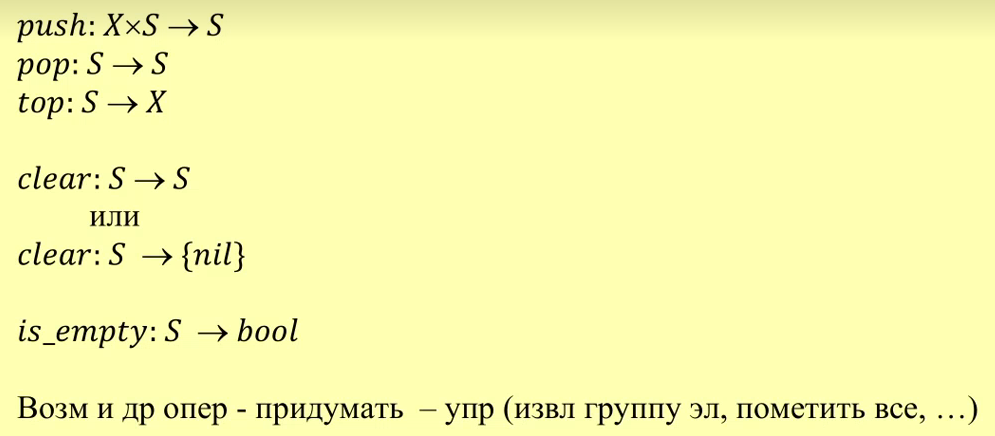
\includegraphics[width=0.7\linewidth]{pictures/5_1.PNG}
    \item
      \textbf{Аксиомы:}\\
      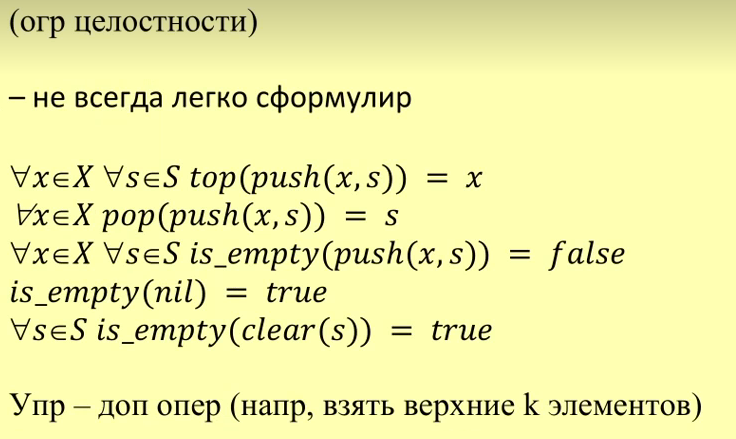
\includegraphics[width=0.7\linewidth]{pictures/5_2.PNG}
  \end{itemize}

  \textbf{Прикладная программа:} \\
   Массивы (статические или динамические), динамические структуры данных и прочее.\\ \\
  
  \textbf{Определение новых типов данных на основе более простых (иерархия типов)}\\
   Имея некоторый базовый тип можно строить производные типы и реализовывать их различным образом.\\
   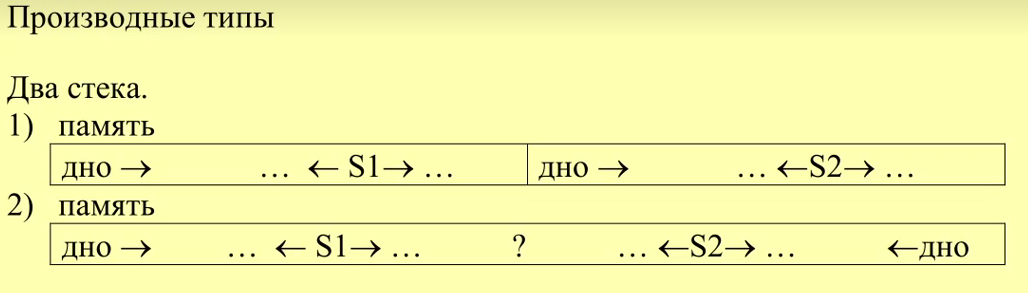
\includegraphics[width=0.7\linewidth]{pictures/5_3.PNG}\\ \\

  \textbf{Предметная область:} \\
  \textbf{Очередь} - одномерная однородная структура данных с "обычными" операциями над очередью (или абстрактный тип данных, реализованный по принципе  FIFO (first-in-first-out))). \\ \\
  
  Примеры:\\

  \begin{itemize}
    \item Очередь в кассу (идеализированная) 
    \item Tруба
  \end{itemize} \\

  Применение:\\

  \begin{itemize}
    \item В системах массового обслуживания для моделирования доступа к ресурсу
    \item В операционных системах для моделирования доступа к ресурсу
    \item Для организации каналов передачи данных
  \end{itemize}

  Определение АТД (абстрактного типа данных) \textbf{очередь} состоит из трех частей:\\

  \begin{itemize}
    \item 
      \textbf{Множества данных:}\\
      Множество простых/базовых данных обозначим Х\\
      Множество всех очередей обозначим queue или Q
    \item
      \textbf{Множество операций над стеками:}\\ 
      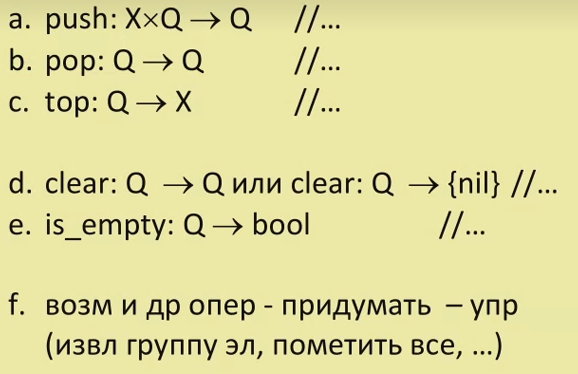
\includegraphics[width=0.7\linewidth]{pictures/5_4.PNG}
    \item
      \textbf{Аксиомы:}\\
      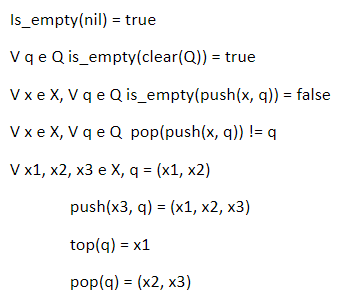
\includegraphics[width=0.7\linewidth]{pictures/5_5.PNG}
  \end{itemize}\\

  \textbf{Дек} – абстрактный тип данных, являющийся обобщение очереди и стека – последовательность, открытая для изменения с двух сторон.\\

  \textbf{Пример реализации стека на языке программирования Java:}\\ \\
  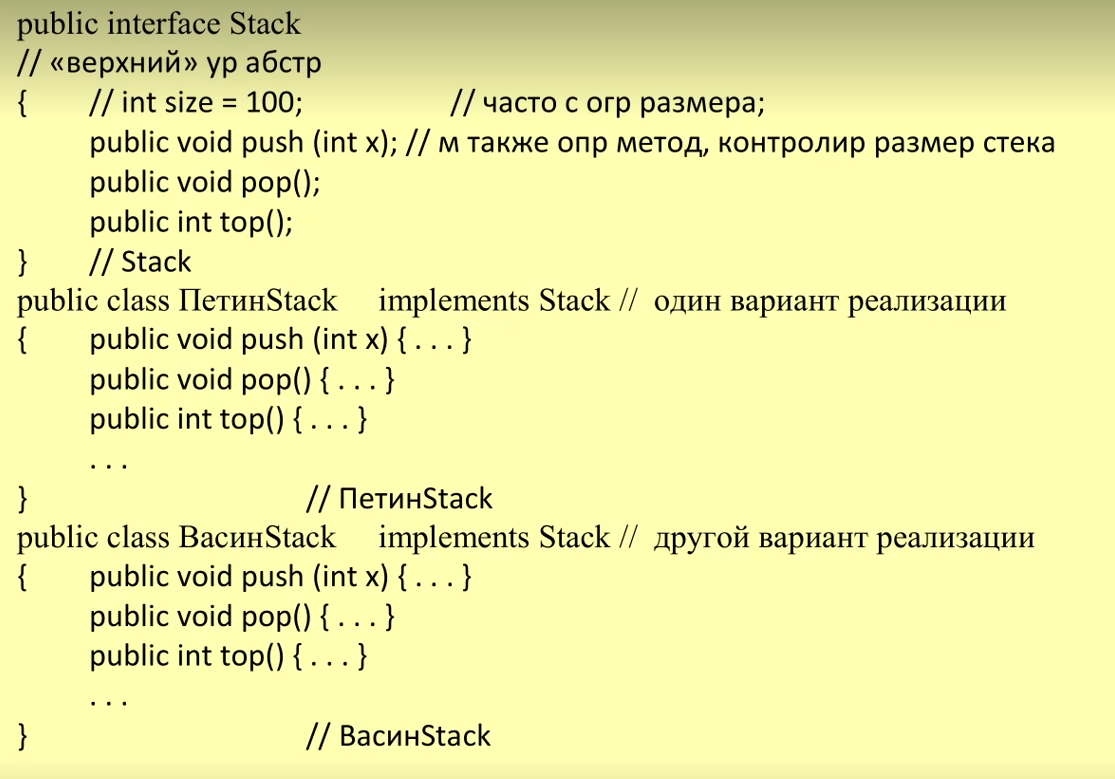
\includegraphics[width=0.7\linewidth]{pictures/5_6.PNG}\\ \\

  \textbf{Вычисление выражений в ОПЗ}\\
  \url{https://habr.com/ru/post/100869/}\\
  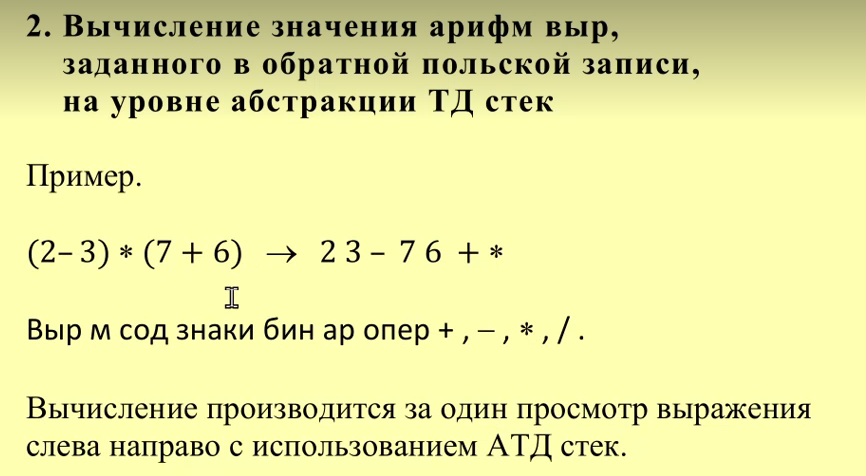
\includegraphics[width=0.7\linewidth]{pictures/5_7.PNG}\\
  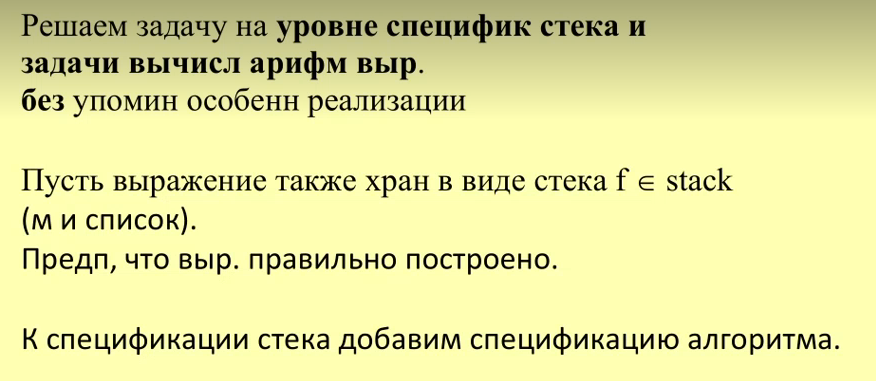
\includegraphics[width=0.7\linewidth]{pictures/5_8.PNG}\\
  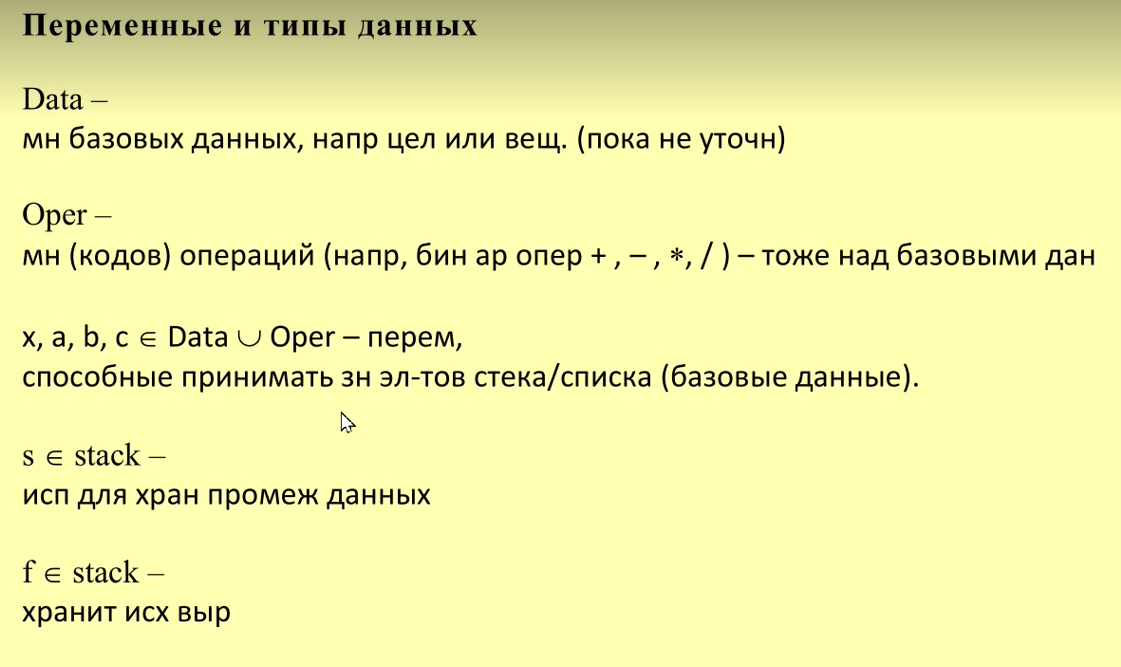
\includegraphics[width=0.7\linewidth]{pictures/5_9.PNG}\\
  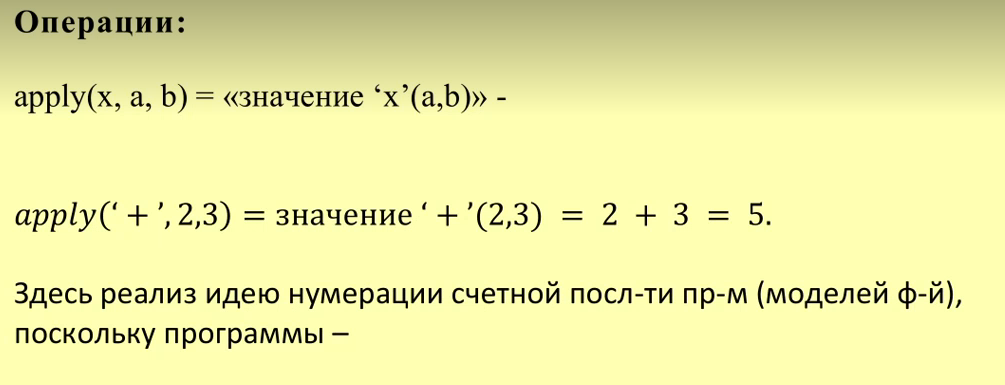
\includegraphics[width=0.7\linewidth]{pictures/5_10.PNG}\\
  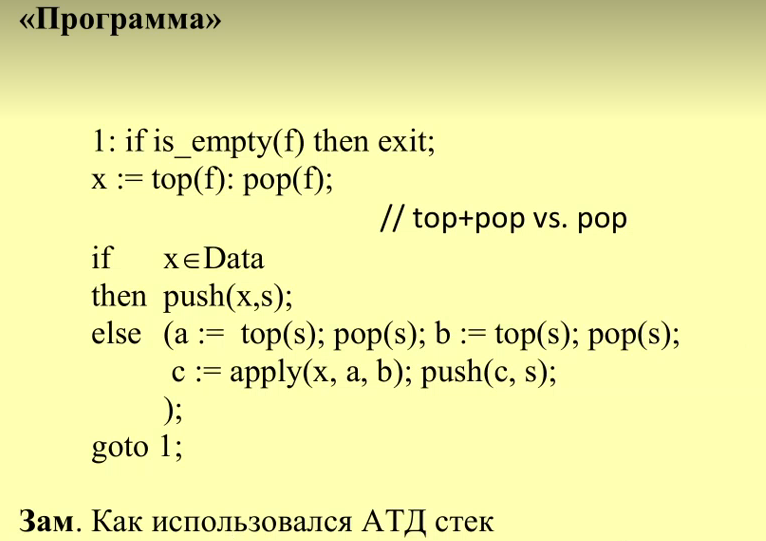
\includegraphics[width=0.7\linewidth]{pictures/5_11.PNG}\\
